\begin{recipe}
    [% 
        preparationtime = {\unit[1]{h}},
        portion = {\portion{2}},
        bakingtime = {\unit[40]{min}},
        source = {whiteplate.com}
    ]
    {Roast pepper and cheese galette}

    \introduction{%
        Whenever I think about fancy dinner (supper?), I reach for stuffed pastry.
        Ladies and gentlemen, tonight we're serving French galette!
    }
    % TODO: check if rendered properly
    \ingredients{%
        \unit[200]{g} & Flour \\
        \nicefrac{1}{4} tbs. & Salt \\
        \unit[100]{g} & Butter \\
        \unit[100]{g} & Sour cream \\
        \textbf{Filling} &  \\
        2 & Pepper \\
        1 & Garlic clove \\
        \unit[100]{g} & Ricotta \\
        \unit[50]{g} & Cheese (eg.
        Grana Padano) \\
        \unit[50]{g} & Mozzarella \\
        & Fresh basil
    }

    \preparation{%
        \step Mix flour, salt and cold butter.
        Add sour cream and quickly knead the dough.
        If needed, add spoon or two of cold water.
        \underline{Cover with foil and refrigerate for an hour.}

        \step Roast slices of pepper (30 min, \unit[200]{\textcelcius})

        \step In a bowl, mix garlic and olive oil, salt and pepper to taste.

        \step On bench covered with flour, stretch the dough to form a circle, place it on parchment.
        In the middle (leaving about 5 cm edge) spread ricotta, mozzarella and Grana Padano.
        Place pepper on the cheese, starting with the outer edge of the cheesy filling.

        \step  Wrap free edges towards the centre (see picture).

        \step Bake for 30-40 min.

        \step Garnish with basil leaves.
    }

    \hint{%
        If the dough is very gluey, wet your hands for easier handling.
    }

\end{recipe}
\begin{figure}[h]
    \centering
    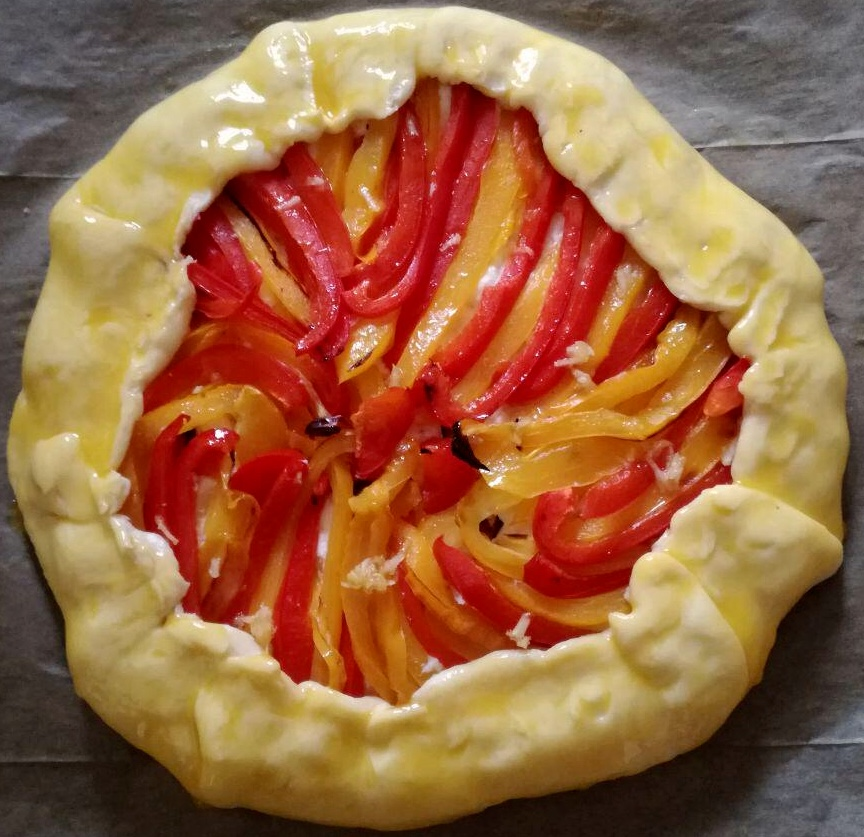
\includegraphics[width=8cm]{pic/galette}
\end{figure}
\begin{figure}[h]
    \centering
    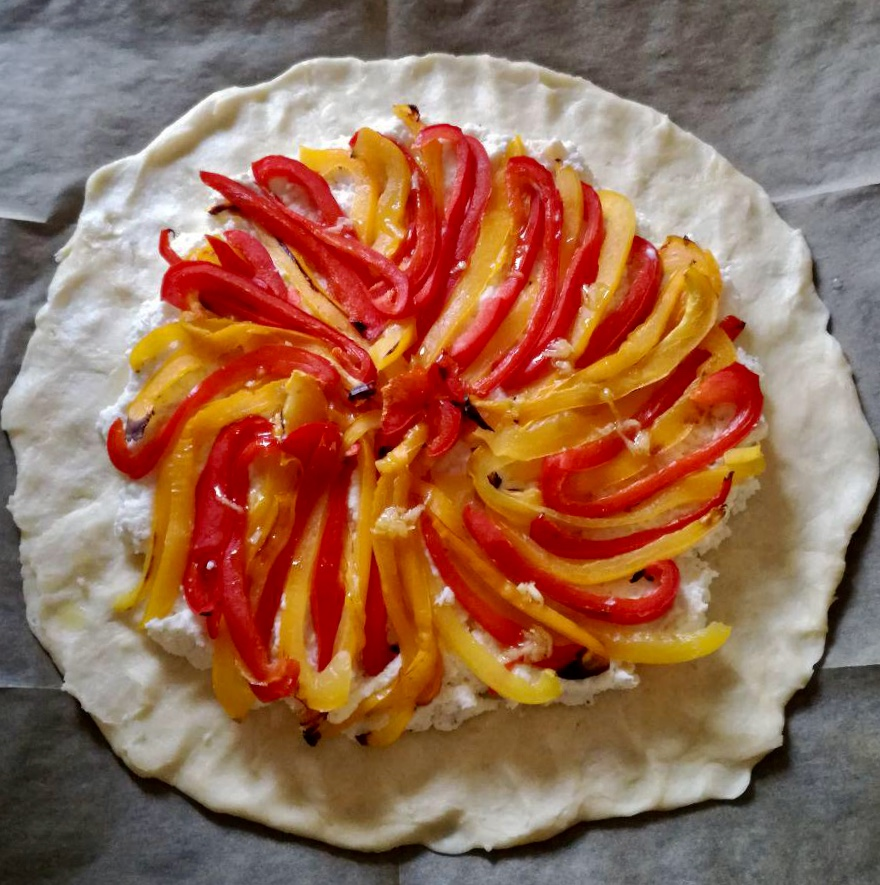
\includegraphics[width=8cm]{pic/galette_2}
\end{figure}
% TODO: alongside